\documentclass[12pt, a4paper]{article}
\usepackage[a4paper, includeheadfoot, mag=1000, left=2cm, right=1.5cm, top=1.5cm, bottom=1.5cm, headsep=0.8cm, footskip=0.8cm]{geometry}
% Fonts
\usepackage{fontspec, unicode-math}
\setmainfont[Ligatures=TeX]{CMU Serif}
\setmonofont{CMU Typewriter Text}
\usepackage[english, russian]{babel}
% Indent first paragraph
\usepackage{indentfirst}
\setlength{\parskip}{5pt}
% Diagrams
\usepackage{graphicx}
\usepackage{float}
% Page headings
\usepackage{fancyhdr}
\pagestyle{fancy}
\renewcommand{\headrulewidth}{0pt}
\setlength{\headheight}{16pt}
%\newfontfamily\namefont[Scale=1.2]{Gloria Hallelujah}
\fancyhead{}

\usepackage{amsmath}

\graphicspath{ {./images/} }

\usepackage{listings}
\lstdefinestyle{lablisting}{
  basicstyle=\scriptsize\ttfamily,
  numbers=left,
  stepnumber=1,
  otherkeywords={EOF, O\_RDONLY, STDIN\_FILENO, STDOUT\_FILENO, STDERR\_FILENO},
  numbersep=10pt,
  showspaces=false,
  showstringspaces=false
}

\newcommand{\specialcell}[2][l]{%
  \begin{tabular}[#1]{@{}l@{}}#2\end{tabular}}

\begin{document}

% Title page
\begin{titlepage}
\begin{center}

\textsc{Федеральное государственное автономное образовательное учреждение высшего\\
образования "Национальный исследовательский университет ИТМО"}
\vfill
\textbf{Лабораторная работа №6\\[4mm]
по дисципение "Информационная безопасность"\\[4mm]
Расшифрование криптограммы на основе эллиптических кривых\\[4mm]
}
\textit{Вариант 10\\[20mm]}
\begin{flushright}
Выполнил: студент Саржевский И.А.
\\[2mm]Группа: P3402\\[4mm]
Преподаватель: к.т.н., доцент\\
Маркина Т.А.
\end{flushright}
\vfill
г. Санкт-Петербург\\[2mm]
2021 г.

\end{center}
\end{titlepage}

\begin{huge}Лабораторная работа №6\end{huge}\\[4mm]
\begin{Large}Расшифрование криптограммы на основе эллиптических\\кривых\end{Large}\\

\section*{Цель работы}

Расшифровать текст, используя приведенный алфавит на основе кривой
$E_{751}(-1,1): y^2=x^3-1x+1\:(mod\:751)$.

\section*{Задание}

Алгоритм шифрования на основе эллиптических кривых состоит из следующих шагов:

\begin{enumerate}
  \item Случайным образом выбирается секретный ключ $n_b$;
  \item Вычисляется публичный ключ $P_b = n_bG$;
  \item Выбирается случайное число $k$;
  \item Рассчитывается $kG$;
  \item Рассчитывается $P_m + kP_b$, где $P_m$ - исходное сообщение;
  \item Пара $(kG; P_m + kP_b)$ составляет зашифрованное сообщение.
\end{enumerate}

Чтобы расшифровать сообщение, получателю необходимо рассчитать значение $n_bkG$,
и вычесть его из $P_m + kP_b$.

Разработанная программа принимает путь к yaml-файлу, в котором описаны исходные
данные: секретный ключ $n_b$ и последовательность пар точек, представляющих
зашифрованное сообщение.

\section*{Исходные данные}

\lstinputlisting[style=lablisting]{../src/var10.yaml}

\section*{Листинг разработанной программы}

\subsubsection*{elliptic\_curve.rs}

\lstinputlisting[style=lablisting]{../src/elliptic_curve.rs}

\subsubsection*{main.rs}

\lstinputlisting[style=lablisting]{../src/main.rs}

\section*{Результаты работы программы}

\begin{figure}[H]
    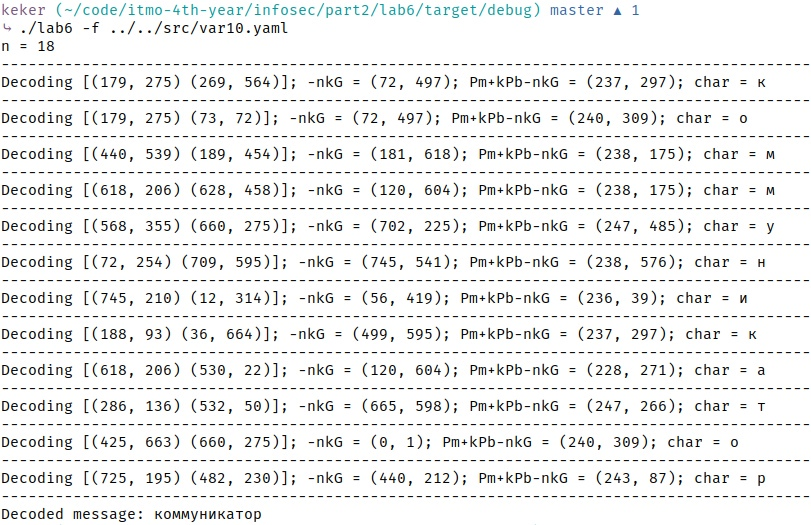
\includegraphics[scale = 0.6]{res}
    \caption{Результат работы программы}
    \centering
\end{figure}

\section*{Вывод}

В результате выполнения данной лабораторной работы был изучен алгоритм
дешифрации текста на основании эллиптических кривых и реализована
программа, позволяющая расшифровать криптограмму, используя приведенный
алфавит на основе кривой
$E_{751}(-1,1): y^2=x^3-1x+1\:(mod\:751)$.

\end{document}
